\documentclass{article}
\usepackage{graphicx}
\usepackage{amsfonts}
\usepackage{enumitem}
\usepackage{pmboxdraw}
\usepackage{nicematrix}
\usepackage[T1]{fontenc}
\usepackage{lmodern}
\usepackage{microtype}
\usepackage{multicol}
\usepackage[dvipsnames]{xcolor}
\usepackage{eso-pic}
\usepackage{booktabs}
\usepackage{menukeys}
\renewmenumacro{\menu}{angularmenus}
\renewmenumacro{\keys}{shadowedangularkeys}
\renewmenumacro{\directory}{pathswithfolder}
\usepackage{ccicons}
\usepackage{tikz}
\usepackage{pgfplots}
\usepgfplotslibrary{polar}
\pgfplotsset{compat=1.18}
\definecolor{linkcolor}{RGB}{40, 70, 120}
\usepackage{caption}
\usepackage[top=1in, bottom=1in, left=1in, right=1in]{geometry}
\usepackage{colortbl}
\newtheorem{theorem}{Theorem}
\usepackage{tcolorbox}
\usepackage{float}
\tcbuselibrary{listings}
\usetikzlibrary{decorations.pathreplacing, calligraphy}
\tcbuselibrary{skins, breakable}
\usepackage{bm}
\usepackage{mdframed}
\usepackage{tocloft}
\usepackage{minted}
\usepackage{titlesec}
\setminted[bash]{
    style=tango,
    breaklines=true,
    frame=single,
    framesep=0mm,
    rulecolor=\color{gray},
    bgcolor=black!5,
    fontsize=\small,
    numbers=left,
    numbersep=5pt
}
\definecolor{codebg}{gray}{0.93}
\newcommand{\code}[1]{\colorbox{codebg}{\texttt{#1}}}
\titleformat{\section}
  {\Large\bfseries\scshape}{\thesection.}{0.5em}{}[\titlerule]
\titleformat{\subsection}
  {\large\bfseries\scshape}{\thesubsection.}{0.5em}{}
  [\vspace{1pt}\hspace{2em}\rule{\dimexpr\textwidth-2em\relax}{0.4pt}]

\titleformat{\subsubsection}
  {\normalsize\bfseries\scshape}{\thesubsubsection.}{0.5em}{}
  [\vspace{1pt}\hspace{4em}\rule{\dimexpr\textwidth-4em\relax}{0.4pt}]
\renewcommand{\cftsecleader}{\cftdotfill{\cftdotsep}} 
\usetikzlibrary{calc}
\newmdenv[linewidth=2pt, linecolor=black!60, topline=false, bottomline=false, rightline=false, backgroundcolor=teal!5!white, frametitle={\small\textbf{Definition}},
frametitlefont=\small\bfseries]{definition}
\newcounter{exercise}
\newcommand{\exercise}{%
  \stepcounter{exercise}%
  \noindent\textbf{Exercise \theexercise.}\quad
}
\newtcolorbox{callout}[1]{
  enhanced,
  colback=calloutbg,
  colframe=calloutborder,
  fonttitle=\bfseries\normalsize,
  title={#1},
  boxrule=0.6pt,
  arc=2pt,
  left=10pt, right=10pt, top=6pt, bottom=6pt,
  borderline west={3pt}{0pt}{calloutborder},
}
\definecolor{inkblack}{HTML}{1A1A1A}
\definecolor{stepblue}{HTML}{1E3A5F}
\definecolor{ruleblue}{HTML}{2E6DA4}
\definecolor{calloutbg}{HTML}{F4F7FB}
\definecolor{calloutborder}{HTML}{2E6DA4}

% Colors
\definecolor{terminalgray}{HTML}{808080}
\definecolor{terminalgreen}{HTML}{00FF00} 
\definecolor{terminalred}{HTML}{FF0000} 

% Terminal style box
\newtcblisting{linuxterminal}{
    colback=black,
    coltext=white,
    colframe=black,
    arc=0mm,
    width=1\textwidth, % Increased width to fit longer lines
    center,               % Centers the oversized box on the page
    top=3mm,
    bottom=3mm,
    left=2mm,
    right=2mm,
    listing only,
    listing options={
        basicstyle=\ttfamily\small,
        breaklines=true,
        columns=fullflexible,
        keepspaces=true,
        escapeinside={(*}{*)}
    }
}

% Styled components

\newcommand{\gbox}[1]{%
\textcolor{terminalgray}{[}%
\makebox[2.5em] [c]{\textcolor{terminalgreen}{#1}}%
\textcolor{terminalgray}{]}%
}

\newcommand{\rbox}[1]{%
\textcolor{terminalgray}{[}%
\makebox[8.5em][c]{\textcolor{terminalred}{#1}}%
\textcolor{terminalgray}{]}%
}

\newcommand{\graytext}[1]{\textcolor{terminalgray}{#1}}
\newcommand{\errtext}[1]{\textcolor{terminalred}{#1}}
\newcommand{\spc}{\hspace{3.7em}}


\usepackage[colorlinks=true, urlcolor=linkcolor, linkcolor=black]{hyperref}



\begin{document}
 
 \begin{titlepage}

\AddToShipoutPictureBG*{%
  \AtPageLowerLeft{%
    \begin{tikzpicture}[overlay, remember picture]
      
      \draw[line width=2pt, color=black!80, rounded corners=15pt] 
        ($(current page.south west) + (0.5in,0.5in)$) 
        rectangle 
        ($(current page.north east) - (0.5in,0.5in)$);
      
      \draw[line width=0.7pt, color=black!60, rounded corners=12pt] 
        ($(current page.south west) + (0.55in,0.55in)$) 
        rectangle 
        ($(current page.north east) - (0.55in,0.55in)$);
    \end{tikzpicture}%
  }%
}
\begin{center}
\hspace{0pt}\\
\vspace{4cm}
{\Large \textbf{Principal Author}: \textit{\href{https://www.reddit.com/u/Significant-Wrap-589/s/LexVz3vvN0}{u/Significant-Wrap-589}}}\\[5pt]
{\Large \textbf{Co-Author \& Document Designer}: \textit{\href{https://www.reddit.com/u/MurkyUnit3180/s/QuyAn31plr}{u/MurkyUnit3180}}}\\[3cm]
{\scalebox{2}{\Huge\bfseries LINUX}}\\
\vspace{0.8cm}
{\LARGE\bfseries A BRIEF GUIDE TO}\\[10pt]
{\LARGE\bfseries GAMING}\\

\vfill
    {\normalsize\itshape A community guide by \href{https://www.reddit.com/r/Indiangamers}{r/Indiangamers}}\\[4pt]
    {\small Version 1.0 \(\cdot\) May 2026 \(\cdot\) Licensed under \ccbysa~4.0} \\[2pt]
    {\small\textit{This guide is a living document and will be updated over time.}}
\end{center}
\end{titlepage}

\clearpage
\phantomsection
\pdfbookmark{\contentsname}{toc}
\tableofcontents
\vspace{1em} 
\hrule
\clearpage

\section{What is Linux?}

At its most precise, Linux is not an operating system; it is a kernel. The \textit{kernel} is the core program that sits between your hardware and everything else running on your machine. It manages the CPU, memory, storage, and peripheral devices. As the GNU Project puts it:

\begin{mdframed}[linewidth=1.5pt, linecolor=black!50, topline=true, bottomline=true,
  leftline=false, rightline=false, backgroundcolor=black!3]
  \small\itshape
  ``Linux is the kernel: the program in the system that allocates the machine's resources to the other programs that you run. The kernel is an essential part of an operating system, but useless by itself.''\\[4pt]
  \normalfont\small --- \href{https://www.gnu.org/gnu/linux-and-gnu.en.html}{GNU Project, gnu.org}
\end{mdframed}

\noindent What most people call ``Linux'' is more accurately a \textbf{GNU/Linux distribution}, the kernel bundled with system software, a package manager, a desktop environment,
and various tools that make it a complete, usable OS.

According to \href{https://www.kernel.org/linux.html}{kernel.org}, Linux was originally written from scratch by Linus Torvalds as a Unix-like system, targeting POSIX compliance, with support for true multitasking, virtual memory, and shared libraries. It was first developed for 32-bit x86 PCs but today runs on virtually every processor architecture in existence.

\subsection{How a Linux System Is Structured}

A complete Linux system consists of several layers:

\begin{itemize}[leftmargin=1.5em, nosep, label={\tiny\textbullet}]
  \item \textbf{Bootloader}: loads the OS on startup (e.g.\ GRUB)
  \item \textbf{Kernel}: manages hardware, memory, and processes
  \item \textbf{Init system}: bootstraps user space after boot (typically \code{systemd})
  \item \textbf{Shell}: your interface to the system (e.g.\ \code{bash}, \code{zsh})
  \item \textbf{Desktop Environment}: the graphical layer (e.g.\ GNOME, KDE Plasma)
  \item \textbf{Package Manager}: installs and manages software
\end{itemize}

\begin{tcolorbox}[arc=12pt, outer arc=10pt, 
colback=blue!4!white, colframe=blue!40!black, title=\textbf{Kernel $\neq$ OS}]
 If someone hands you ``the Linux kernel'', you cannot use it as a desktop system. You need a full \textit{distribution}, which packages the kernel with everything else. When people say they ``run Linux'', they mean a distribution like Ubuntu, Arch, or Fedora.
\end{tcolorbox}

\subsection{What is a Distribution?}

A \textbf{distribution} (or \textit{distro}) is a complete operating system built around the Linux kernel. Different distros make different choices about which desktop environment, package manager, and software to include. The kernel itself is the same, only what surrounds it differs. Common package managers you will encounter:

\begin{itemize}[leftmargin=1.5em, nosep, label={\tiny\textbullet}]
  \item \code{apt}: Debian, Ubuntu, Pop!\_OS
  \item \code{dnf}: Fedora
  \item \code{pacman}: Arch Linux, Manjaro
\end{itemize}

\noindent To update your system, the command looks like this depending on your distro:

\begin{minted}{bash}
# Debian/Ubuntu
sudo apt update && sudo apt upgrade

# Fedora
sudo dnf upgrade

# Arch
sudo pacman -Syu

\end{minted}

\noindent Keeping your system updated is not optional, it is the foundation of a stable gaming setup. On Linux, drivers, compatibility layers like \textit{Proton}, and core libraries like \textit{glibc} and \textit{Mesa} all ship through the package manager. An outdated system means outdated graphics drivers, which directly translates to lower performance, crashes, or games outright refusing to launch.

Unlike Windows, where driver updates are fragmented across manufacturer websites and Windows Update, Linux consolidates everything into a single command. Your GPU driver, kernel, and game runtime dependencies all update together.

\begin{tcolorbox}[arc=12pt, outer arc=10pt, colback=red!5!white, colframe=red!60!black, title=\textbf{Warning}]
Never run a partial upgrade. On Arch, \code{pacman -Sy package} without a full \code{-Syu} first can break your system by introducing dependency mismatches.
\end{tcolorbox}

\subsection{Why Linux Matters}

Linux may occupy a modest share of consumer desktops, but it quietly runs the world. \textit{Every} major cloud provider (AWS, Google Cloud, and Microsoft Azure) runs
Linux as their foundational operating system. As of 2025, Linux powers 90\% of public cloud infrastructure, 100\% of the world's top 500 supercomputers, and 77\% of all web server deployments worldwide.

\begin{callout}{\textbf{By the Numbers (2025)}}
  \begin{itemize}[nosep, leftmargin=1.2em, label={\tiny\textbullet}]
    \item \textbf{90\%} of public cloud infrastructure runs Linux
    \item \textbf{100\%} of TOP500 supercomputers run Linux
    \item \textbf{78.5\%} of developers use Linux as a primary or secondary platform
    \item \textbf{96.4\%} of production Kubernetes clusters run on Linux
  \end{itemize}
\end{callout}

\noindent The phone in your pocket almost certainly runs Android, which is built on the Linux kernel. The servers that stream your games, process your payments, and host
your favourite websites run Linux. It is certainly the backbone of modern computing.

For the end user, what this means is stability, transparency, and control. Linux is free, open-source, and maintained by thousands of contributors worldwide. No forced telemetry or licence fees.

\subsection{Linux and Gaming}

Linux gaming has undergone a fundamental shift since Valve released \textit{Proton} in 2018. Proton is a compatibility layer developed by Valve in collaboration with \href{https://www.codeweavers.com}{CodeWeavers}, built on top of \textit{Wine}, that translates Windows API calls into Linux-compatible equivalents. In plain terms: it lets you run Windows games on Linux with little to no configuration.

\begin{figure}[htbp]
\centering
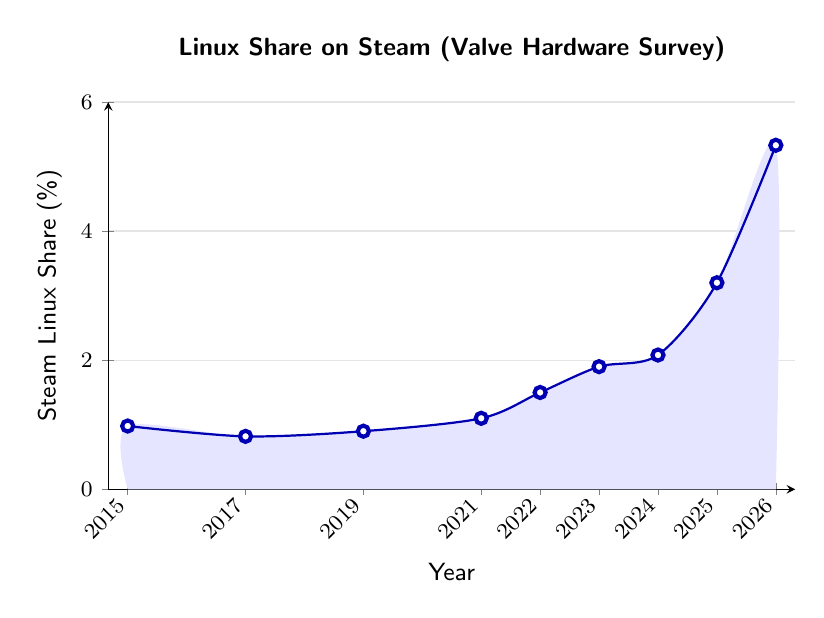
\begin{tikzpicture}
\begin{axis} [
    width=0.85\textwidth,
    height=6.5cm,
    title={\textbf{Linux Share on Steam (Valve Hardware Survey)}},
    title style={yshift=5pt, font=\small\sffamily},
    xlabel={Year},
    ylabel={Steam Linux Share (\%)},
    label style={font=\small\sffamily},
    xtick={2015,2017,2019,2021,2022,2023,2024,2025,2026},
    xticklabel style={rotate=45, anchor=east, font=\footnotesize\sffamily, /pgf/number format/1000 sep={}},
    yticklabel style={font=\footnotesize\sffamily},
    ymin=0, ymax=6,
    axis x line=bottom,
    axis y line=left,
    ymajorgrids=true,
    grid style={line width=0.5pt, draw=gray!20},
    enlarge x limits=0.03,
]


\addplot [
    draw=none,
    fill=blue!10,
    forget plot,
    smooth
] coordinates {
    (2015, 0) (2015, 0.98)
    (2017, 0.82)
    (2019, 0.90)
    (2021, 1.10)
    (2022, 1.50)
    (2023, 1.90)
    (2024, 2.08)
    (2025, 3.20)
    (2026, 5.33) (2026, 0)
};


\addplot [
    color=blue!70!black,
    thick,
    mark=*,
    mark options={fill=white, draw=blue!70!black, line width=1.5pt, mark size=2pt},
    smooth
] coordinates {
    (2015, 0.98)
    (2017, 0.82)
    (2019, 0.90)
    (2021, 1.10)
    (2022, 1.50)
    (2023, 1.90)
    (2024, 2.08)
    (2025, 3.20)
    (2026, 5.33)
};

\end{axis}
\end{tikzpicture}

\vspace{2mm}
{\footnotesize\sffamily\color{gray} Source: \href{https://steampowered.com}{Valve Steam Hardware \& Software Survey}}
\end{figure}



The release of the Steam Deck in 2022 accelerated this significantly. Running Valve's own \textit{SteamOS}, a Linux-based operating system, the Steam Deck proved that Linux could run a serious gaming library on consumer hardware. As of November 2025, \textit{Proton 10.0-3} is the latest stable release, bringing fixes and expanded support across thousands of titles including
\textit{God of War Ragnar\"{o}k}, \textit{Marvel's Spider-Man Remastered}, and more.

\begin{tcolorbox}[arc=12pt, outer arc=10pt,
  colback=blue!4!white, colframe=blue!40!black,
  title=\textbf{How Proton Works}]
  A Windows game makes calls to \textbf{DirectX} and the \textbf{Windows API}. \textit{Proton} intercepts these calls and translates them in real time using \textbf{DXVK} (DirectX $\rightarrow$ Vulkan) and \textbf{Wine} (Windows API $\rightarrow$ Linux). The game never knows it is not running on Windows.
\end{tcolorbox}

\noindent That said, Linux gaming is not without its caveats. Games with aggressive
kernel-level anti-cheat (such as Valorant's Vanguard or PUBG's BattlEye in certain configurations) remain the primary blocker. This is an active area of
development, and compatibility improves with every \textit{Proton} release.

\begin{tcolorbox}[arc=12pt, outer arc=10pt,
  colback=red!5!white, colframe=red!60!black,
  title=\textbf{Anti-Cheat Warning}]
  Before switching, check your most-played games on
  \href{https://www.protondb.com}{ProtonDB} and \href{https://areweanticheatyet.com}{areweanticheatyet.com}. Kernel-level anti-cheat is the one area where Linux genuinely cannot help you, yet.
\end{tcolorbox}

\newpage \section{Installing Linux}

This guide uses \textit{CachyOS} as the recommended distribution.
\href{https://cachyos.org}{CachyOS} is an Arch-based rolling-release distribution that bundles all necessary gaming libraries, Proton, and dependencies into a single
meta-package install, making it one of the most convenient starting points for Linux gaming without sacrificing access to the full Arch ecosystem.
\begin{callout}{\textbf{Why Not Ubuntu or Fedora?}}
  Both are solid distros. CachyOS is chosen here purely for its convenience ---
  one meta-package gets you a complete gaming setup. That is the only reason.
\end{callout}

\subsection{Choosing a Distro}

With hundreds of Linux distributions available, the choice can feel overwhelming. For
this guide, the decision has already been made: \textbf{CachyOS}. This subsection
explains why, and briefly covers the alternatives worth knowing about.

\subsubsection{Why CachyOS?}

\href{https://cachyos.org}{CachyOS} is an Arch-based rolling-release distribution. Its primary advantage for this guide is convenience: gaming libraries, Proton, and
all necessary dependencies are available as a single meta-package, meaning the gap between a fresh install and a working gaming setup is minimal.

Being Arch-based is also a practical advantage: Valve built SteamOS on Arch, meaning kernel-level fixes and gaming improvements from Valve tend to trickle down to
Arch-based distros like CachyOS naturally.

\subsubsection{Alternatives Worth Knowing}

CachyOS is not the only valid choice. The following are the most relevant alternatives:

\begin{itemize}[leftmargin=1.5em, label={\tiny\textbullet}, nosep]
  \item \textbf{Bazzite}: Fedora-based, immutable, excellent out-of-the-box gaming
    experience. Recommended for users who want something that simply works with minimal
    configuration. The safer choice for beginners.
  \item \textbf{Nobara}: Fedora-based, created by the developer of Proton-GE.
    Gaming tools pre-installed, good hardware support.
  \item \textbf{EndeavourOS}: Arch-based, minimal, close to vanilla Arch but with
    a friendlier installer. Less opinionated than CachyOS.
  \item \textbf{Ubuntu / Linux Mint}: Debian-based, highly stable, large community. Not gaming-optimized, but reliable and well-documented.
\end{itemize}

\begin{tcolorbox}[arc=12pt, outer arc=10pt,
  colback=blue!4!white, colframe=blue!40!black,
  title=\textbf{Rolling Release vs.\ Stable Release}]
  CachyOS is a \textbf{rolling release}, packages update continuously rather than
  in fixed version cycles. This means you always have the latest drivers and software,
  which matters for gaming. The trade-off is that updates occasionally introduce
  breakage. This guide covers basic troubleshooting for exactly that reason.
\end{tcolorbox}

\subsection{Preparing the Installation Medium}

Before Linux can be installed, a bootable installation medium must exist. Traditional tools such as \textit{Rufus} or \textit{balenaEtcher} flash a single ISO directly onto a USB drive; which works, but comes with a significant limitation: every time a different ISO is needed, the drive must be reformatted and rewritten from scratch.

This guide takes a different approach. Since a fallback Windows installer is useful to have on hand, in case anything goes wrong, both the CachyOS and Windows 11
ISOs will live on the same USB drive simultaneously. This is made possible by \textit{Ventoy}.

\href{https://www.ventoy.net}{Ventoy} installs a small bootloader onto the USB once.
After that, any number of ISO files can simply be copied onto the drive like normal
files. On boot, Ventoy presents a menu and lets you choose which ISO to launch.
No reflashing required.

\subsubsection{Downloads}

Before proceeding, download the following:

\begin{itemize}[nosep, leftmargin=1.5em, label={\tiny\textbullet}]
  \item \textbf{Ventoy} (Windows installer):
    \href{https://www.ventoy.net/en/download.html}{ventoy.net/en/download.html}
  \item \textbf{CachyOS Desktop Edition ISO}:
    \href{https://cachyos.org/download/}{cachyos.org/download}
  \item \textbf{Windows 11 Disk Image}:
    \href{https://www.microsoft.com/en-us/software-download/windows11}{microsoft.com}
\end{itemize}

\subsubsection{Installing Ventoy}

\begin{enumerate}[nosep, leftmargin=1.5em, label={\arabic*.}]
  \item Plug in your USB drive
  \item Extract the downloaded \code{Ventoy\_windows.zip} and open
    \code{Ventoy2Disk.exe}
  \item Your USB drive should appear in the device list
  \item Click Install, Ventoy will write its bootloader to the drive
  \item Once complete, open \directory{This PC} in Windows File Explorer
  \item Copy both ISO files directly onto the USB drive, no extraction needed
\end{enumerate}

\begin{tcolorbox}[arc=12pt, outer arc=10pt,
  colback=red!5!white, colframe=red!60!black,
  title=\textbf{Warning}]
  Installing Ventoy will erase all existing data on the USB drive. Back up anything important before proceeding. A USB drive of at least \textbf{16 GB} is recommended
  to fit both ISOs comfortably.
\end{tcolorbox}

\subsection{Booting into CachyOS}

With the USB prepared, the next step is to tell your PC to boot from it rather than the internal drive. This is done through the \textit{BIOS} or \textit{UEFI} firmware
settings, a low-level interface that controls hardware behaviour before the OS loads.

\subsubsection{Entering the BIOS}

\begin{enumerate}[leftmargin=1.5em, nosep, label={\arabic*.}]
  \item Plug in the USB drive
  \item Restart your PC
  \item As soon as the screen turns on, repeatedly press the BIOS entry key for your
    device. Common keys are \keys{F2}, \keys{Delete}, \keys{F10}, or \keys{F12}, the exact key varies by manufacturer and can be found with a quick search for your device model
\end{enumerate}

\begin{callout}{\textbf{Common BIOS Entry Keys by Manufacturer}}
  \begin{itemize}[leftmargin=1.5em, nosep, label={\tiny\textbullet}]
    \item \textbf{ASUS}: \keys{Delete} or \keys{F2}
    \item \textbf{MSI}: \keys{Delete}
    \item \textbf{Gigabyte}: \keys{Delete} or \keys{F2}
    \item \textbf{Dell}: \keys{F2} or \keys{F12}
    \item \textbf{HP}: \keys{F10} or \keys{Esc}
    \item \textbf{Lenovo}: \keys{F2} or \keys{Fn} + \keys{F2}
  \end{itemize}
\end{callout}

\subsubsection{Configuring Boot Order}

Once inside the BIOS:

\begin{enumerate}[leftmargin=1.5em, nosep, label={\arabic*.}]
 \item Navigate to a tab labelled \menu{Boot}, \menu{Boot Options}, or \menu{Boot Priority}, the exact name varies by firmware
  \item Move your USB device to the top of the boot order, above the internal drive
  \item Locate the Secure Boot option and set it to Disabled
  \item Press \keys{F10} to save and exit. Or navigate to \menu{Exit, Save Changes and Exit}
\end{enumerate}

\begin{tcolorbox}[arc=12pt, outer arc=10pt,
  colback=red!5!white, colframe=red!60!black,
  title=\textbf{Why Disable Secure Boot?}]
  Secure Boot is a firmware security feature that only allows signed bootloaders to
  run. While CachyOS supports Secure Boot, disabling it avoids potential complications
  during installation and is the recommended approach for a first-time Linux install.
  It can be re-enabled after setup if needed.
\end{tcolorbox}

\subsubsection{Selecting the CachyOS ISO in Ventoy}

After saving BIOS settings, your PC will restart and boot into the Ventoy menu:

\begin{enumerate}[leftmargin=1.5em, nosep, label={\arabic*.}]
  \item Use \keys{\arrowkeyup} and \keys{\arrowkeydown} to navigate to the CachyOS ISO
  \item Press \keys{\return} to boot into it
  \item CachyOS will load into a live environment, nothing is installed yet
\end{enumerate}

\subsection{The Installation Process}

With CachyOS booted from the Ventoy menu, the installation can begin. This subsection walks through every step of the Calamares installer sequentially, following the
\href{https://wiki.cachyos.org}{official CachyOS documentation}.

\subsubsection{Don't Panic; Boot Messages}

As the ISO loads, you will likely see a screen full of rapidly scrolling white text on a black background. This is normal.  

\begin{mdframed}[linewidth=1.5pt, linecolor=black!50, topline=true, bottomline=true,
  leftline=false, rightline=false, backgroundcolor=black!3]
  \small\itshape
  Linux briefly displays system initialisation messages before the graphical desktop
  starts. Unlike Windows, which conceals this process behind splash screens and
  animations, Linux exposes it. These are kernel and \code{systemd} messages logged
  in real time as hardware is detected and services are started.\\[4pt]
  \normalfont\small --- Behaviour described in the
  \href{https://wiki.archlinux.org/title/Systemd/Journal}{Arch Wiki: systemd/Journal}
  and \href{https://www.debian.org/doc/manuals/debian-reference/ch03.en.html}{Debian
  Reference, Chapter 3: System Initialisation}
\end{mdframed}

\noindent What you are seeing is \code{systemd}, the init system responsible for bootstrapping the user space after the kernel loads. When the kernel executes \code{systemd} as process 1, it takes over system initialisation,
orchestrating service startup, dependency tracking, and system management. Every line of text is a service starting, a device being detected, or a filesystem
being mounted. It looks chaotic. It is not.

The messages are produced by \code{systemd-journald}, the journal service that
logs both kernel and system messages, either into persistent binary
data below \directory{/var/log/journal} or into volatile binary data below
\directory{/run/log/journal/}. Once installed, you can review any boot's
messages at any time with: \begin{minted}{bash}
journalctl -b     # current boot messages
journalctl -b -1  # previous boot messages
\end{minted}


\begin{linuxterminal}
(*\graytext{Starting}*) Apply Kernel Variables...
(*\gbox{OK}*) Mounted Temporary /etc/pacman.d/gnupg directory.
(*\gbox{OK}*) Mounted Temporary directory /tmp.
(*\rbox{20.480467}*) vmwgfx 0000:00:02.0: [drm] (*\errtext{\string*ERROR\string*}*) vmwgfx seems to be running on an unsupported hypervisor.
(*\rbox{20.480475}*) vmwgfx 0000:00:02.0: [drm] (*\errtext{\string*ERROR\string*}*) This configuration is likely broken.
(*\rbox{20.480478}*) vmwgfx 0000:00:02.0: [drm] (*\errtext{\string*ERROR\string*}*) Please switch to a supported graphics device to avoid problems.
(*\gbox{OK}*) (*\graytext{Finished}*) Apply Kernel Variables.
(*\spc*) (*\graytext{Starting}*) Network Management...
(*\spc*) (*\graytext{Starting}*) Network Name Resolution...
(*\gbox{OK}*) Started Network Management.
(*\spc*) (*\graytext{Starting}*) Enable Persistent Storage in systemd-networkd...
(*\spc*) (*\graytext{Starting}*) Wait for Network to be Online...
(*\gbox{OK}*) Started Network Name Resolution.
(*\gbox{OK}*) (*\graytext{Reached target}*) Host and Network Name Lookups.
(*\gbox{OK}*) (*\graytext{Listening on}*) Load/Save RF Kill Switch Status /dev/rfkill Watch.
(*\spc*) (*\graytext{Starting}*) Virtual Console Setup...
(*\gbox{OK}*) Stopped Virtual Console Setup.
(*\spc*) (*\graytext{Starting}*) Virtual Console Setup...
(*\gbox{OK}*) (*\graytext{Finished}*) Enable Persistent Storage in systemd-networkd.
(*\gbox{OK}*) Stopped Virtual Console Setup.
(*\spc*) (*\graytext{Starting}*) Virtual Console Setup...
(*\gbox{OK}*) (*\graytext{Finished}*) Virtual Console Setup.
(*\gbox{OK}*) (*\graytext{Finished}*) Wait for udev To Complete Device Initialization.
(*\gbox{OK}*) (*\graytext{Reached target}*) ZFS pool import target.
(*\spc*) (*\graytext{Starting}*) Mount ZFS filesystems...
(*\gbox{OK}*) (*\graytext{Finished}*) Mount ZFS filesystems.
(*\gbox{OK}*) (*\graytext{Reached target}*) Local File Systems.
(*\gbox{OK}*) (*\graytext{Listening on}*) Boot Loader Control Service Socket.
(*\gbox{OK}*) (*\graytext{Listening on}*) System Extension Image Management.
(*\spc*) (*\graytext{Starting}*) Automatic Boot Loader Update...
(*\spc*) (*\graytext{Starting}*) Create System Files and Directories...
(*\spc*) (*\graytext{Starting}*) Load JSON user/group Records from Credentials...
(*\gbox{OK}*) (*\graytext{Finished}*) Automatic Boot Loader Update.
(*\gbox{OK}*) (*\graytext{Finished}*) Load JSON user/group Records from Credentials.
(*\gbox{OK}*) (*\graytext{Finished}*) Create System Files and Directories.
(*\spc*) (*\graytext{Starting}*) Rebuild Dynamic Linker Cache...
(*\spc*) (*\graytext{Starting}*) Initial Setup...
(*\spc*) (*\graytext{Starting}*) Rebuild Journal Catalog...
(*\spc*) (*\graytext{Starting}*) Record System Boot/Shutdown in UTMP...
(*\gbox{OK}*) (*\graytext{Finished}*) Record System Boot/Shutdown in UTMP.
(*\gbox{OK}*) (*\graytext{Finished}*) Initial Setup.
(*\gbox{OK}*) (*\graytext{Reached target}*) First Boot Complete.
(*\spc*) (*\graytext{Starting}*) Save Transient machine-id to Disk...
(*\gbox{OK}*) (*\graytext{Finished}*) Rebuild Journal Catalog.
(*\gbox{OK}*) (*\graytext{Finished}*) Save Transient machine-id to Disk.
(*\rbox{$\ast\ast\ast$}*) (3 of 3) A start job is running for Rebuild Dynamic Linker Cache (16s / no limit)
\end{linuxterminal}

\begin{multicols}{2}
\begin{center}
\begin{tabular}{@{}ll@{}}
\toprule
\textbf{Prefix} & \textbf{Meaning} \\
\midrule
\code{[  OK  ]} & Started successfully \\
\code{[ INFO ]} & Informational \\
\code{[~~~*~~~]} & Starting, wait \\
\bottomrule
\end{tabular}
\end{center}

\columnbreak

\begin{center}
\begin{tabular}{@{}ll@{}}
\toprule
\textbf{Prefix} & \textbf{Meaning} \\
\midrule
\code{[FAILED]} & Ignorable on live ISO \\
\code{[WARNING]} & Non-critical \\
\code{[DEPENDS]} & Waiting on another service \\
\bottomrule
\end{tabular}
\end{center}
\end{multicols}

\noindent Wait for the messages to finish. The graphical desktop will load
automatically. Once it does, you will be greeted by the \textbf{CachyOS Hello} window.

\begin{figure}[htbp]
  \centering
  \includegraphics[width=0.85\textwidth]{01.png}
  \caption*{\small\textit{CachyOS live desktop with Hello window on first boot}}
\end{figure}

\subsubsection{Network Connectivity}

Before launching the installer, a stable internet connection is required for the
online installation mode, which downloads the latest packages during install.

\begin{enumerate}[leftmargin=1.5em, nosep, label={\arabic*.}]
  \item Locate the \textbf{network tray icon} in the bottom-right corner of the taskbar
  \item Click it --- your available Wi-Fi networks will appear
  \item Select your network and enter your password
  \item Confirm connectivity before proceeding
\end{enumerate}

\begin{tcolorbox}[arc=12pt, outer arc=10pt,
  colback=red!5!white, colframe=red!60!black,
  title=\textbf{Warning}]
  Do not launch the installer on an unstable connection. If the download stalls at
  33\% progress, it is almost always a network issue --- not a system failure. The
  \href{https://wiki.cachyos.org/cachyos_basic/faq/}{official CachyOS FAQ} confirms this is the most common installation failure point.
\end{tcolorbox}

\noindent Once connected, click \textbf{Launch Installer} in the CachyOS Hello window. The Calamares installer will open.

\subsubsection{Language}

The first tab of Calamares asks for your preferred language. Select it from the list
and click \textbf{Next}.

\subsubsection{Timezone and Location}

Select your timezone from the map or the dropdown. This sets your system clock
correctly and determines locale defaults. Click \textbf{Next}.

\subsubsection{Keyboard Layout}

Select your keyboard layout. If you are unsure, the default for your selected region
is usually correct. Use the test field at the bottom of the screen to verify. Click
\textbf{Next}.

\subsubsection{Bootloader}

\begin{callout}{\textbf{What is a Bootloader?}}
  A bootloader is the software that runs before the operating system loads. It
  presents a menu where you select which OS to boot into. Windows has its own
  bootloader, \textbf{Windows Boot Manager}, but hides it behind splash
  screens. Linux exposes it directly and gives you the choice.
\end{callout}

\vspace{0.5em}

CachyOS offers two bootloader choices:

\begin{itemize}[leftmargin=1.5em, label={\tiny\textbullet}, nosep]
  \item \textbf{Limine} (recommended); a portable, modern bootloader and the
    reference implementation of the Limine boot protocol. According to the
    \href{https://wiki.cachyos.org/cachyos_basic/changelogs/gui_installer/}{CachyOS
    installer changelog}, Limine is now the default and ships with automatic Btrfs
    snapshot support out of the box
  \item \textbf{GRUB}, the GNU GRand Unified Bootloader, the traditional Linux
    standard. More compatible with dual-boot setups and older hardware, but does not
    offer automatic snapshot integration
\end{itemize}

\textbf{Choose Limine} for this guide and click \textbf{Next}.

\begin{callout}{\textbf{What are Snapshots?}}
  Snapshots are point-in-time copies of a filesystem. If a system update breaks
  something, you can boot a previous snapshot and restore your system to its last
  working state. Think of them as save states --- if something goes wrong, load the
  previous save.
\end{callout}

\subsubsection{Partitioning}

This guide assumes a full, dedicated Linux install, no dual boot. Select
\textbf{Erase Disk}.

\begin{tcolorbox}[arc=12pt, outer arc=10pt,
  colback=red!5!white, colframe=red!60!black,
  title=\textbf{Warning}]
  Erase Disk permanently deletes everything on the selected drive. Back up your
  Windows data before proceeding. Confirm you have selected the correct disk.
  If multiple drives are present, disconnect any you do not want wiped.
\end{tcolorbox}

\noindent After selecting Erase Disk, you will be prompted to choose a filesystem:

\begin{itemize}[leftmargin=1.5em, label={\tiny\textbullet}, nosep]
  \item \textbf{Btrfs} (recommended); supports snapshots natively. Combined with
    Limine, gives you automatic rollback capability. Calamares auto-detects whether
    your drive is an SSD or HDD and adjusts mount options accordingly
  \item \textbf{ext4}, the classic stable Linux filesystem. Widely supported, no
    snapshot capability
  \item \textbf{XFS}, high performance, good for large files, no snapshots
\end{itemize}

\begin{tcolorbox}[arc=12pt, outer arc=10pt,
  colback=blue!4!white, colframe=blue!40!black,
  title=\textbf{What is a Filesystem?}]
  A filesystem is the method by which an operating system organises and stores data
  on a drive. Linux supports multiple filesystems, Btrfs, ext4, XFS among others.
  Windows uses \textbf{NTFS}. Linux can read NTFS drives, but installing Linux itself
  on an NTFS partition is not supported or recommended.
\end{tcolorbox}

\noindent Select \textbf{Btrfs} and click \textbf{Next}.

\subsubsection{Desktop Environment}

\begin{tcolorbox}[arc=12pt, outer arc=10pt,
  colback=blue!4!white, colframe=blue!40!black,
  title=\textbf{Desktop Environment vs.\ Window Manager}]
  A \textbf{Desktop Environment} (DE) is a complete, integrated desktop experience ---
  file manager, settings app, notification tray, lock screen, and more, all packaged
  together. Think of it as a fully furnished house. Examples: KDE Plasma, GNOME, XFCE.\\[6pt]
  A \textbf{Window Manager} (WM) controls only window behaviour --- resizing, tiling,
  keyboard shortcuts. Think of it as the bare structure of a house with no furniture;
  you build everything yourself. Examples: Hyprland, niri, i3. Every DE ships with a
  WM already included --- KDE uses KWin, GNOME uses Mutter.
\end{tcolorbox}

\noindent For this guide, choose a Desktop Environment. Tiling window managers like
Hyprland are powerful but not appropriate for a first Linux install.

The available options for beginners:

\begin{itemize}[leftmargin=1.5em, label={\tiny\textbullet}, nosep]
  \item \textbf{KDE Plasma} (recommended): modern, feature-rich, highly
    customizable. Workflow is similar to Windows. The default choice for this guide
  \item \textbf{GNOME}: minimal, opinionated, clean. Closer in feel to macOS than
    Windows. A different workflow that takes adjustment
  \item \textbf{XFCE}: lightweight and efficient. Recommended only for older
    hardware with limited RAM
\end{itemize}

\begin{callout}{\textbf{Note}}
  There is no objectively best Desktop Environment. The difference is workflow.
  KDE is the starting point for most beginners due to its similarity to Windows and
  its depth of customization options. You are not locked in; CachyOS supports
  multiple DEs installed simultaneously, and you can switch later.
\end{callout}

\noindent Select \textbf{KDE Plasma} and click \textbf{Next}.

\begin{figure}[htbp]
  \centering
  \includegraphics[width=0.85\textwidth]{02.png}
  \caption*{\small\textit{Desktop Environment selection in Calamares}}
\end{figure}

\subsubsection{Packages}

Calamares will present a package selection screen. Ensure the default selections are
checked, these include the base KDE packages and essential system components.
Do not uncheck anything unless you know what you are removing. Click \textbf{Next}.

\subsubsection{Users}

Fill in the following fields:

\begin{itemize}[leftmargin=1.5em, nosep, label={\tiny\textbullet}, nosep]
  \item \textbf{Your name}: display name, can be anything
  \item \textbf{Username}: your login name, lowercase, no spaces
  \item \textbf{Computer name}: the hostname of your machine on the network
  \item \textbf{Password}: used for login and every \code{sudo} command. Do not
    forget this
\end{itemize}

\begin{tcolorbox}[arc=12pt, outer arc=10pt,
  colback=red!5!white, colframe=red!60!black,
  title=\textbf{Warning}]
  Your password is required for every administrative action on the system. There is
  no password recovery prompt like Windows --- if you forget it, recovery requires
  booting into a live environment and manually resetting it. Write it down somewhere
  safe.
\end{tcolorbox}

\subsubsection{Summary and Installation}

Calamares will display a full summary of your chosen configuration, language,
timezone, bootloader, filesystem, desktop, and username. Review everything carefully.
If anything is incorrect, use the \textbf{Back} button to correct it.

When satisfied, click \textbf{Install}. The installer will begin writing to disk.
Depending on your internet connection and drive speed, this takes between
\textbf{30 minutes and 2 hours}.

\begin{callout}{\textbf{During Installation}}
  Do not close the installer, put the machine to sleep, or disconnect from the
  internet while installation is in progress. An interrupted install can leave the
  drive in an unbootable state.
\end{callout}

\subsubsection*{What Happens During Installation}

At around 30\%, the copying of files is completed, this takes the longest. After
that, the installer creates users, removes live-system-specific packages, installs
additional packages, removes language packs and drivers not needed for your hardware,
and sets up the bootloader. On a network install, time depends entirely on your internet speed and mirror proximity.

\begin{callout}{\textbf{Progress Stages}}
  The progress bar is not linear. It will appear to stall. According to the \href{https://wiki.cachyos.org/cachyos_basic/faq/}{official CachyOS FAQ}, stalling
  at 33\% is almost always a network or mirror issue, not a system failure. Wait at
  least five minutes before concluding something is wrong.
\end{callout}

\subsubsection*{If Installation Fails}

If an installation fails, the installer may not properly unmount partitions, meaning continuous errors can occur if you attempt to reinstall
immediately. Always reboot back into the live ISO before trying again.

\subsubsection*{After Installation Completes}

When the installer finishes, Calamares will prompt you to restart. Remove the USB
drive when instructed and press \keys{\return}. Your system will boot into the
\textbf{Limine} bootloader menu, a clean interface showing your installed operating
systems. Select \textbf{CachyOS} and press \keys{\return}.

\noindent You are now running CachyOS. Section~3 covers what to do immediately
after first boot.

\begin{figure}[H]
\centering

% Define a sophisticated, cohesive color palette
\definecolor{nordBlue}{HTML}{5E81AC}
\definecolor{nordGreen}{HTML}{A3BE8C}
\definecolor{nordOrange}{HTML}{D08770}
\definecolor{gridGray}{HTML}{E5E9F0}
\definecolor{textDark}{HTML}{2E3440}
\definecolor{textMuted}{HTML}{4C566A}

% Ensure you have \usepackage{booktabs} and \usepackage{colortbl} in your preamble
\begin{tikzpicture}
\begin{polaraxis}[
    width=0.75\textwidth,
    % Configure clean, dashed background grids
    grid=both,
    grid style={line width=0.5pt, draw=gridGray, dashed},
    % Axis Limits and Ticks
    ymin=0, ymax=5,
    ytick={1,2,3,4,5},
    yticklabels={1,2,3,4,5},
    yticklabel style={font=\tiny\color{textMuted}, fill=white, inner sep=1pt},
    % Five-point star layout (360 / 5 = 72 degree increments)
    xtick={0, 72, 144, 216, 288},
    xticklabels={
        Snapshot\\Support,
        Raw\\Performance,
        Data\\Integrity,
        Stability,
        Recovery
    },
    % Multi-line text alignment for clear spacing
    xticklabel style={font=\small\color{textDark}, align=center, inner sep=8pt},
    % Clean, borderless horizontal legend placed cleanly underneath the chart
    legend style={
        at={(0.5,-0.15)},
        anchor=north,
        legend columns=-1,
        draw=none,
        fill=none,
        font=\small\color{textDark},
        /tikz/every even column/.append style={column sep=15pt}
    },
]

% --- Btrfs ---
\addplot[
    line width=1.5pt,
    color=nordBlue,
    fill=nordBlue,
    fill opacity=0.2,
    mark=*,
    mark size=2pt,
    mark options={fill=white, line width=1.5pt}
] coordinates {
    (0,   5)
    (72,  3)
    (144, 5)
    (216, 4)
    (288, 4)
    (360, 5)
};
\addlegendentry{Btrfs}

% --- ext4 ---
\addplot[
    line width=1.5pt,
    color=nordOrange,
    fill=nordOrange,
    fill opacity=0.2,
    mark=*,
    mark size=2pt,
    mark options={fill=white, line width=1.5pt}
] coordinates {
    (0,   0)
    (72,  5)
    (144, 3)
    (216, 5)
    (288, 4)
    (360, 0)
};
\addlegendentry{ext4}

% --- XFS ---
\addplot[
    line width=1.5pt,
    color=nordGreen,
    fill=nordGreen,
    fill opacity=0.2,
    mark=*,
    mark size=2pt,
    mark options={fill=white, line width=1.5pt}
] coordinates {
    (0,   0)
    (72,  5)
    (144, 3)
    (216, 5)
    (288, 3)
    (360, 0)
};
\addlegendentry{XFS}

\end{polaraxis}
\end{tikzpicture}

\vspace{8mm}

% Beautiful companion data table using booktabs structure
\small
\renewcommand{\arraystretch}{1.2} % Extra breathing room for rows
\begin{tabular}{lccccc}
    \toprule
    \color{textDark}Filesystem & Snapshot & Performance & Integrity & Stability & Recovery \\
    \midrule
    \color{nordBlue}Btrfs      & 5 & 3 & 5 & 4 & 4 \\
    \color{nordOrange}ext4     & 0 & 5 & 3 & 5 & 4 \\
    \color{nordGreen}XFS       & 0 & 5 & 3 & 5 & 3 \\
    \bottomrule
\end{tabular}

\vspace{6mm}
\begin{minipage}{0.85\textwidth}
    \centering
    {\fontsize{8.5pt}{11pt}\selectfont\color{textMuted}
    Qualitative comparison based on \href{https://linuxjournal.com}{Linux Journal},
    \href{https://linuxano.com}{Linuxano}, and \href{https://vps.do}{VPS.DO} filesystem
    analyses (2025--2026). Scores reflect desktop gaming use case priorities.\par}
\end{minipage}
\end{figure}

\subsection{Post-Install Checks}

The first boot into a fresh CachyOS install is not the time to start installing games.
Before anything else, the system needs to be verified, updated, and confirmed healthy.
Skipping these steps is how systems end up in broken states two weeks later.

\subsubsection{Update the System}

Open a terminal. On KDE Plasma, press \keys{META} or search for
\textbf{Konsole} in the application launcher. Run:

\begin{minted}{bash}
sudo pacman -Syu
\end{minted}

This synchronizes the package database and upgrades all installed packages. On a
fresh online install the list will be short. On an offline install, expect a
significantly larger download.

\begin{tcolorbox}[arc=12pt, outer arc=10pt,
  colback=red!5!white, colframe=red!60!black,
  title=\textbf{Warning}]
  Never run \code{pacman -Sy} or \code{pacman -Sy package} without the \code{u}
  flag. A partial upgrade on Arch-based systems introduces dependency
  mismatches that can break the entire system. Always use \code{-Syu}.
\end{tcolorbox}

\subsubsection{Verify paru; Your AUR Helper}

The \textbf{Arch User Repository} (AUR) is a community-maintained repository of
build scripts for software not available in the official Arch repositories. It is one
of the biggest practical advantages of using an Arch-based system. Nearly any
software you can think of has an AUR package.

To use the AUR, you need an \textbf{AUR helper}. CachyOS ships with
\href{https://github.com/morganamilo/paru}{\code{paru}}, a feature-rich AUR helper
written in Rust, installed by default. Confirm it is present:

\begin{minted}{bash}
paru --version
\end{minted}

If it prints a version number, \code{paru} is ready. If the terminal returns
\code{command not found}, install it manually:

\begin{minted}{bash}
sudo pacman -S --needed base-devel
git clone https://aur.archlinux.org/paru.git
cd paru
makepkg -si
\end{minted}

\begin{tcolorbox}[arc=12pt, outer arc=10pt,
  colback=blue!4!white, colframe=blue!40!black,
  title=\textbf{paru vs pacman}]
  \code{paru} is a wrapper around \code{pacman}. It handles everything \code{pacman}
  does, plus searches and builds AUR packages. The syntax is identical, anywhere
  you would use \code{pacman}, you can use \code{paru} instead. According to the
  \href{https://wiki.cachyos.org/cachyos_basic/faq/}{official CachyOS FAQ}, when AUR
  packages are installed, use \code{paru -Syu} for updates instead of \code{pacman
  -Syu} to ensure AUR packages are upgraded as well.
\end{tcolorbox}

\begin{callout}{\textbf{A Note on Graphical Package Managers}}
  The \href{https://wiki.cachyos.org/cachyos_basic/faq/}{official CachyOS FAQ}
  explicitly warns against using \textbf{Pamac} for system package management.
  It is known to improperly handle certain package management tasks, such as
  corrupting system keyrings, leading to PGP signature errors that prevent future
  updates. Use \code{pacman} or \code{paru} from the terminal for system updates.
\end{callout}

\subsubsection{Enable Multilib}

\textbf{Multilib} is a repository that provides 32-bit libraries on a 64-bit system.
It is required for Steam, many games, and Wine. On CachyOS it is typically enabled
by default, but verify it is active by opening the \directory{/etc/pacman.conf}:

\begin{minted}{bash}
sudo nano /etc/pacman.conf
\end{minted}

Scroll down and confirm the following lines are present and \textbf{uncommented}
(no \code{\#} at the start):

\begin{minted}{bash}
[multilib]
Include = /etc/pacman.d/mirrorlist
\end{minted}

If they are commented out, remove the \code{\#} characters, save with
\keys{Ctrl+O}, and exit with \keys{Ctrl+X}. Then sync:

\begin{minted}{bash}
sudo pacman -Syu
\end{minted}

\subsubsection{Verify GPU Drivers}

Before launching any games, confirm your GPU drivers are correctly loaded. Run:

\begin{minted}{bash}
	glxinfo | grep "OpenGL renderer"
\end{minted}

The output should display your GPU name, for example:

\begin{minted}{bash}
	OpenGL renderer string: NVIDIA GeForce RTX 3070/PCIe/SSE2
\end{minted}

\begin{tcolorbox}[arc=12pt, outer arc=10pt,
	colback=red!5!white, colframe=red!60!black,
	title=\textbf{Warning}]
	If the output shows \code{llvmpipe} or \code{softpipe}, the correct GPU drivers
	are not loaded. These are software renderers. Games will run at a fraction of
	their normal performance or not at all. Do not proceed to gaming setup until this
	is resolved.
\end{tcolorbox}

\noindent If \code{glxinfo} is not found, install it with:

\begin{minted}{bash}
	sudo pacman -S mesa-utils
\end{minted}

\subsubsection{Check Critical systemd Services}

Confirm that essential services are running correctly:

\begin{minted}{bash}
	systemctl --failed
\end{minted}

A healthy system returns an empty list. If any services appear as \code{failed},
investigate them individually:

\begin{minted}{bash}
	systemctl status service-name
\end{minted}

\begin{callout}{\textbf{NetworkManager}}
	The most common failed service on a fresh install is \code{NetworkManager}.
	If your network is working, it is running. This is sometimes a display artefact.
	Verify with:
	\begin{minted}{bash}
		systemctl status NetworkManager
	\end{minted}
	It should show \code{active (running)}.
\end{callout}

\noindent With the system updated, \code{paru} confirmed, multilib enabled, GPU
drivers verified, and services healthy, the system is ready. Section~3 covers
the first boot experience and initial desktop configuration.

%─────────────────────────────────────────────────────────────────────────────
\newpage
\section{First Boot}

You have successfully installed CachyOS. This section walks through the first boot
sequence, the login screen, and getting comfortable with your new desktop environment
before touching anything system-critical.

\subsection{The Limine Screen}

After removing the USB and rebooting, your system will present the \textbf{Limine}
bootloader menu. Use \keys{\arrowkeyup} and \keys{\arrowkeydown} to navigate to
\textbf{CachyOS} and press \keys{\return}.

\subsection{The Login Screen}

You will be greeted by a graphical login screen. This is the \textbf{display manager}
--- a program that provides a graphical login interface, handles user authentication,
and launches your chosen desktop environment.

\begin{tcolorbox}[arc=12pt, outer arc=10pt,
	colback=blue!4!white, colframe=blue!40!black,
	title=\textbf{What is a Display Manager?}]
	The display manager is the first graphical program that runs after boot. It starts
	the graphical environment, presents a login screen, authenticates the user, and
	then hands control to the desktop environment --- in this case, KDE Plasma. CachyOS
	uses \textbf{SDDM} (Simple Desktop Display Manager) by default.
\end{tcolorbox}

\noindent Type the password you set during installation and press \keys{\return}.

\subsection{Welcome to Linux}

CachyOS will greet you with the \textbf{CachyOS Hello} window --- a graphical tool
for post-install configuration, system tweaks, and package installation. You will
return to it later. For now, set it aside.

\subsection{Making Yourself at Home}

Before doing anything system-critical, spend a few minutes becoming comfortable
with the desktop. This is not wasted time --- familiarity with the UI makes
everything that follows easier.

\subsubsection{Changing the Wallpaper}

\begin{enumerate}[leftmargin=1.5em, nosep, label={\arabic*.}]
	\item Right-click on the desktop
	\item Select \menu{Desktop and Wallpaper} or press \keys{Ctrl+Shift+D}
	\item Choose a preloaded wallpaper, or add your own using the \textbf{Add} button
\end{enumerate}

\subsubsection{Customising the Panel}

\begin{enumerate}[leftmargin=1.5em, nosep, label={\arabic*.}]
	\item Right-click the bottom panel
	\item Select \menu{Show Panel Configuration}
	\item Adjust layout, widgets, and position to your preference
\end{enumerate}

\subsubsection{Things Worth Trying}

\begin{itemize}[leftmargin=1.5em, label={\tiny\textbullet}, nosep]
	\item Verify all keyboard shortcuts and keys are working. Customise them via
	\menu{System Settings, Shortcuts}
	\item Take a screenshot with \keys{PrtSc}
	\item Explore \menu{System Settings, Display and Monitor} to configure refresh
	rate and scaling
	\item Explore \menu{System Settings, Appearance} --- KDE ships with thousands
	of community-made themes, icon packs, and window decorations
\end{itemize}

\subsection{The Terminal}

On Linux, the terminal is not optional. It is the primary tool for system
administration, package management, and troubleshooting. A
\textbf{terminal emulator} is the graphical application that provides a window
for text input. Inside it runs a \textbf{shell}, the actual command interpreter
that reads your input and instructs the OS what to do.

\begin{tcolorbox}[arc=12pt, outer arc=10pt,
	colback=blue!4!white, colframe=blue!40!black,
	title=\textbf{Terminal vs.\ Shell}]
	The \textbf{terminal} is the window. The \textbf{shell} is the program running
	inside it. Common shells include \code{bash}, \code{zsh}, and \code{fish}.
	CachyOS uses \textbf{Fish} by default --- a user-friendly shell with
	autocompletion and syntax highlighting out of the box. The terminal emulator
	bundled with CachyOS is \textbf{Alacritty} --- a GPU-accelerated terminal
	built for speed.
\end{tcolorbox}

\noindent To open Alacritty, search for it in the application launcher. Pin it to
the taskbar, you will use it constantly. When Alacritty opens, you will see your system information displayed automatically.
This is \textbf{fastfetch} --- a pre-configured tool that prints a formatted system summary on terminal launch. Run it again at any time with:

\begin{minted}{bash}
	fastfetch
\end{minted}

\begin{figure}[H]
	\centering
	\includegraphics[width=0.85\textwidth]{03.png}
	\caption*{\small\textit{Alacritty terminal showing fastfetch system information output}}
\end{figure}



\begin{callout}{\textbf{Why fastfetch matters}}
	When asking for help on any Linux forum or subreddit, always include a screenshot
	of your fastfetch output. It tells others your distro, kernel version, DE, GPU,
	and RAM at a glance --- essential context for troubleshooting.
\end{callout}

%─────────────────────────────────────────────────────────────────────────────
\newpage
\section{File System}

Linux organises all files under a single unified directory tree rooted at \directory{/}.
Understanding this structure is essential --- knowing where configuration files, logs,
and game data live will save significant time when troubleshooting. This section covers
the official filesystem standard, the directory layout, and how to navigate it both
graphically and through the terminal.

\subsection{The Filesystem Hierarchy Standard}

Every file and directory on a Linux system lives under a single root directory:
\directory{/}. This structure is defined by the \textbf{Filesystem Hierarchy
	Standard} (FHS) --- a specification maintained by the Linux Foundation that defines
the directory layout and contents of Unix-like operating systems.

\begin{mdframed}[linewidth=1.5pt, linecolor=black!50, topline=true, bottomline=true,
	leftline=false, rightline=false, backgroundcolor=black!3]
	\small\itshape
	``This standard consists of a set of requirements and guidelines for file and
	directory placement under UNIX-like operating systems. The guidelines are intended
	to support interoperability of applications, system administration tools,
	development tools, and scripts as well as greater uniformity of these systems.''\\[4pt]
	\normalfont\small ---
	\href{https://refspecs.linuxfoundation.org/FHS_3.0/fhs/index.html}{Filesystem
		Hierarchy Standard 3.0, Linux Foundation}
\end{mdframed}

\noindent All files and directories appear under the root directory \directory{/}, even
if they are stored on different physical or virtual devices.  This is
fundamentally different from Windows, which assigns a drive letter (\directory{C:},
\directory{D:}) to each storage device. On Linux, everything is one unified tree.

\subsection{The Directory Tree}

\begin{minted}{bash}
	/
	├── bin/        # essential binaries (ls, cat, cp...)
	├── boot/       # kernel, initramfs, bootloader
	├── dev/        # device files (disks, USB, TTY...)
	├── etc/        # system-wide configuration files
	├── home/       # user home directories
	│   └── user/
	│       ├── Documents/
	│       ├── Downloads/
	│       └── ...
	├── lib/        # essential libraries for /bin
	├── media/      # auto-mounted removable drives
	├── mnt/        # manual mount points
	├── opt/        # optional/third-party software
	├── proc/       # virtual fs: live kernel & process info
	├── root/       # home directory of the root user
	├── run/        # runtime data (PIDs, sockets)
	├── srv/        # data for services (web, FTP...)
	├── sys/        # virtual fs: hardware & kernel info
	├── tmp/        # temporary files (cleared on reboot)
	├── usr/        # user utilities and applications
	│   ├── bin/    # most user commands live here
	│   ├── lib/    # libraries for /usr/bin
	│   ├── local/  # locally compiled software
	│   └── share/  # shared data (icons, docs, themes)
	└── var/        # variable data
	    ├── log/    # system logs
	    ├── cache/  # application cache
	    └── spool/  # print and mail queues
\end{minted}

{\footnotesize\color{gray} Structure defined by
	\href{https://refspecs.linuxfoundation.org/FHS_3.0/fhs/index.html}{FHS 3.0,
		Linux Foundation}. Identical across all FHS-compliant distributions.}

\begin{tcolorbox}[arc=12pt, outer arc=10pt,
	colback=blue!4!white, colframe=blue!40!black,
	title=\textbf{FHS 3.0}]
	The most recent version of the FHS, version 3.0, was published on March 18,
	2015, and is maintained by the Linux Foundation. Most Linux distributions are
	FHS-compliant, with the notable exception of NixOS, which uses a unique hierarchy
	built around the Nix package manager. 
\end{tcolorbox}
\subsection{Key Directories for Gamers}

Most of what you will interact with as a gamer lives in a small subset of these
directories:

\vspace{0.5em}
{\renewcommand{\arraystretch}{1.3}
	\begin{center}
		\begin{tabular}{@{}ll@{}}
			\toprule
			\textbf{Path} & \textbf{Relevance} \\
			\midrule
			\directory{/home/username/} & Your personal files, game saves, configs \\
			\directory{/home/username/.local/share/Steam} & Steam installation and game library \\
			\directory{/home/username/.steam} & Steam runtime and Proton data \\
			\directory{/etc/} & System-wide configuration files \\
			\directory{/var/log/} & System logs for troubleshooting \\
			\directory{/tmp/} & Temporary files, cleared on reboot \\
			\bottomrule
		\end{tabular}
\end{center}}

\begin{callout}{\textbf{Hidden Files}}
	Files and directories beginning with a \code{.} (dot) are hidden by default ---
	\directory{.steam}, \directory{.config}, \directory{.local}. They are not shown
	by \code{ls} unless you use \code{ls -a}. In Dolphin (KDE's file manager), press
	\keys{Ctrl+H} to toggle their visibility.
\end{callout}

\subsection{\textsc{Navigating with the Terminal}}

Open Alacritty and try the following in order. This is not a reference --- it is a
short walkthrough to build muscle memory.

Start by confirming where you are:

\begin{minted}{bash}
	pwd
\end{minted}

This will print \directory{/home/username} --- your home directory is the default
working directory every time a terminal opens. Now list everything in it:

\begin{minted}{bash}
	ls -a
\end{minted}

Your output will look similar to this:

\begin{minted}{text}
	.cache       .config      .local       .pki
	.var         Desktop      Documents    Downloads
	Music        Pictures     Projects     Public
	Templates    Videos       .bash_logout .bash_profile
	.bashrc      .gtkrc-2.0   .zshrc
\end{minted}

\noindent Entries beginning with \code{.} are hidden files and directories. Configuration
files, shell profiles, and application data. They are invisible by default in both
\code{ls} (without \code{-a}) and in Dolphin (without \keys{Ctrl+H}).

Now navigate into a subdirectory:

\begin{minted}{bash}
	cd Pictures/Screenshots
\end{minted}

\begin{callout}{\textbf{Tab Completion}}
	While typing any path, press \keys{Tab} to autocomplete. If multiple matches exist,
	press \keys{Tab} twice to see them all. Make this a habit --- it prevents typos and
	is significantly faster than typing full paths.
\end{callout}

Once inside \directory{Pictures/Screenshots}, list its contents:

\begin{minted}{bash}
	ls
\end{minted}

To open a file directly from the terminal, type its name. For an image file, your
default viewer will launch:

\begin{minted}{bash}
	xdg-open screenshot.png
\end{minted}

To return home at any point:

\begin{minted}{bash}
	cd ~
\end{minted}

\subsection{\textsc{Navigating with Dolphin}}

\textbf{Dolphin} is KDE's file manager and a capable graphical alternative to the
terminal for everyday file operations. Open it from the taskbar or application
launcher and spend a few minutes exploring --- copy, paste, rename, and move files
the same way you would on Windows.

Useful shortcuts:

\begin{itemize}[leftmargin=1.5em, nosep, label={\tiny\textbullet}]
	\item \keys{Ctrl+H} --- toggle hidden files and folders
	\item \keys{F4} --- open an embedded terminal panel at the current directory
	\item \keys{Ctrl+L} --- focus the path bar for direct path entry
	\item \keys{Alt+Left} / \keys{Alt+Right} --- navigate back and forward
\end{itemize}

\begin{callout}{\textbf{\keys{F4} is Underrated}}
	Pressing \keys{F4} in Dolphin opens a terminal panel locked to the directory you
	are currently browsing. This is the fastest way to drop into a terminal at a
	specific location without typing \code{cd} repeatedly.
\end{callout}

\subsubsection{Useful Commands}

The four commands you will use constantly:

\begin{minted}{bash}
	pwd          # print current working directory
	ls           # list directory contents
	ls -a        # list including hidden files
	cd Pictures  # change into the Pictures directory
	cd ~         # return to home directory
\end{minted}

\subsection{\textsc{Launching Apps from the Terminal}}

Every application on Linux can be launched by typing its name in the terminal:

\begin{minted}{bash}
	firefox     # launch Firefox and see its logs
	steam       # launch Steam with full log output
	vlc         # launch VLC
\end{minted}

This is more than a curiosity --- when an application crashes or behaves unexpectedly,
launching it from the terminal prints its log output in real time. This output is
often the fastest way to diagnose what went wrong, and is what Linux forums and
subreddits will ask you to provide when requesting help.
\newpage
\section{Terminal Basics}

The terminal is the most direct interface between you and the operating system. This
section covers command structure, essential commands, keyboard shortcuts, and piping
--- everything needed to operate confidently from the command line before moving into
package management and system configuration.

\subsection{Why the Terminal?}

The terminal is the most direct interface between you and the operating system. While
graphical tools exist for most tasks, the terminal is faster, scriptable, and always
available --- even when the desktop environment breaks. On a rolling-release
distribution like CachyOS, knowing your way around the terminal is not optional.

\begin{mdframed}[linewidth=1.5pt, linecolor=black!50, topline=true, bottomline=true,
	leftline=false, rightline=false, backgroundcolor=black!3]
	\small\itshape
	``The shell is a command interpreter and programming language that provides the
	user interface to a Linux system. It interprets commands typed by the user
	and translates them into instructions the kernel can execute.''\\[4pt]
	\normalfont\small ---
	\href{https://www.gnu.org/software/bash/manual/bash.html}{GNU Bash Manual,
		gnu.org}
\end{mdframed}

\subsection{Anatomy of a Command}

Every command follows the same structure:

\begin{minted}{bash}
	command  [options]  [arguments]
\end{minted}

For example:

\begin{minted}{bash}
	ls  -la  /home/username
\end{minted}

Where \code{ls} is the command, \code{-la} are options (list all files in long
format), and \directory{/home/username} is the argument (the target directory).
Options beginning with a single dash (\code{-}) are short flags; those with double
dashes (\code{--}) are long-form equivalents:

\begin{minted}{bash}
	ls -a
	ls --all     # identical result
\end{minted}

% Define the Nord color palette
\definecolor{nordBlue}{HTML}{81A1C1}
\definecolor{nordOrange}{HTML}{D08770}
\definecolor{nordGreen}{HTML}{A3BE8C}

	
% Define the Nord color palette
\definecolor{nordBlue}{HTML}{81A1C1}
\definecolor{nordOrange}{HTML}{D08770}
\definecolor{nordGreen}{HTML}{A3BE8C}
\definecolor{nordDark}{HTML}{2E3440}
\definecolor{nordLight}{HTML}{D8DEE9}


	
\begin{center}
		\begin{tikzpicture}[
			box/.style={rounded corners=5pt, inner sep=8pt,
				font=\normalsize\ttfamily\bfseries, minimum width=2.0cm,
				minimum height=0.8cm, align=center},
			labelbox/.style={rounded corners=3pt, inner sep=5pt,
				font=\footnotesize\sffamily, minimum width=2.0cm,
				align=center},
			desc/.style={font=\scriptsize\sffamily\color{black!60},
				text width=2.6cm, align=center},
			arrow/.style={->, >=stealth, thick},
			terminal/.style={font=\small\ttfamily, color=black!70}
			]
			
			% --- LAYER 1: THE TERMINAL PROMPT & COMMAND ---
			% Prompt Prefix
			\node[terminal, anchor=east] (prompt) at (-1.5,0) {\textbf{\color{nordGreen}user@host}\color{black!50}{:}\textbf{\color{nordBlue}\raisebox{-0.5ex}{\~{}}}\color{black!70}{\$}};
			
			% Colored command boxes
			\node[box, fill=nordBlue!20, draw=nordBlue] (cmd) at (0,0) {ls};
			\node[box, fill=nordOrange!20, draw=nordOrange] (opt) at (3.2,0) {-la};
			\node[box, fill=nordGreen!20, draw=nordGreen] (arg) at (7.2,0) {/home/username};
			
			
			% --- LAYER 2: ANATOMY LABELS & DESCRIPTIONS ---
			% Labels
			\node[labelbox, fill=nordBlue!10, draw=nordBlue!40, text=nordBlue] (cmd-lbl) at (0,-1.3) {Command};
			\node[labelbox, fill=nordOrange!10, draw=nordOrange!40, text=nordOrange] (opt-lbl) at (3.2,-1.3) {Option};
			\node[labelbox, fill=nordGreen!10, draw=nordGreen!40, text=nordGreen] (arg-lbl) at (7.2,-1.3) {Argument};
			
			% Dynamic Arrows
			\draw[arrow, draw=nordBlue] (cmd.south) -- (cmd-lbl.north);
			\draw[arrow, draw=nordOrange] (opt.south) -- (opt-lbl.north);
			\draw[arrow, draw=nordGreen] (arg.south) -- (arg-lbl.north);
			
			% Descriptions
			\node[desc, anchor=north] at (cmd-lbl.south) {\vspace{0.1cm}The binary or program execution file};
			\node[desc, anchor=north] at (opt-lbl.south) {\vspace{0.1cm}Switches that modify tool behavior};
			\node[desc, anchor=north] at (arg-lbl.south) {\vspace{0.1cm}The target file, directory, or data};
			
			
			% --- LAYER 3: BRACKET & CONCEPT ---
			% Native TikZ Curly Brace
			\draw[decorate, decoration={calligraphic brace, amplitude=6pt}, thick, black!40]
			(-1.1, 0.6) -- (8.6, 0.6);
			\node[font=\footnotesize\sffamily\bfseries\color{black!60}, anchor=south] at (3.75, 0.9)
			{Input: Standard Execution String};
			
			
			% --- LAYER 4: COMMAND OUTPUT EXPLANATION (NEW) ---
			% Downward flow arrow to output
			\draw[arrow, black!20, line width=1.5pt] (3.75, -2.8) -- (3.75, -3.5);
			
			% Terminal Output Block
			\node[draw=black!20, fill=black!5, rounded corners=3pt, text width=10.5cm, font=\footnotesize\ttfamily, inner sep=10pt, anchor=north] (output) at (3.75, -3.6) {
				\color{black!50}{total 16} \\
				drwxr-xr-x  2 username username 4096 May 15 10:00 \color{nordBlue}{\textbf{.}} \\
				drwxr-xr-x  3 root     root     4096 May 15 09:00 \color{nordBlue}{\textbf{..}} \\
				-rw-r--r--  1 username username  220 May 15 09:00 .bash\_logout \\
				-rw-r--r--  1 username username 3771 May 15 09:00 .bashrc
			};
			
			% Output Label
			\node[font=\tiny\sffamily\color{black!40}, anchor=south east] at (output.south east) {Output (stdout)};
			
		\end{tikzpicture}
\end{center}


\subsection{Essential Commands}

\begin{minted}{bash}
	# Navigation
	pwd                    # print current directory
	cd /etc                # change to /etc
	cd ..                  # go up one directory
	cd ~                   # go to home directory
	
	# Files and directories
	ls -la                 # list all files with details
	mkdir myfolder         # create a directory
	rm file.txt            # delete a file
	rm -rf myfolder        # delete a directory recursively
	cp file.txt backup/    # copy a file
	mv file.txt docs/      # move a file
	cat file.txt           # print file contents
	
	# System
	sudo command           # run command as administrator
	man ls                 # open the manual for ls
	which firefox          # find where a binary lives
	echo $SHELL            # print your current shell
\end{minted}

\begin{tcolorbox}[arc=12pt, outer arc=10pt,
	colback=red!5!white, colframe=red!60!black,
	title=\textbf{Warning}]
	\code{rm -rf} is permanent and irreversible. There is no trash bin. Double-check
	the path before executing. Running \code{rm -rf /} as root deletes the entire
	filesystem. According to the
	\href{https://wiki.archlinux.org/title/Security}{Arch Wiki Security guide}, never
	run commands from the internet without reading and understanding them first.
\end{tcolorbox}

\subsection{Reading Manual Pages}

Every standard Linux command has a manual page:

\begin{minted}{bash}
	man pacman
\end{minted}

Navigate with \keys{\arrowkeyup}/\keys{\arrowkeydown}, search with \keys{/} followed
by a search term, and quit with \keys{q}.

\subsection{Useful Shortcuts}

\begin{center}
	{\renewcommand{\arraystretch}{1.3}
		\begin{tabular}{@{}ll@{}}
			\toprule
			\textbf{Shortcut} & \textbf{Action} \\
			\midrule
			\keys{Ctrl+C} & Kill the running process \\
			\keys{Ctrl+Z} & Suspend the running process \\
			\keys{Ctrl+D} & Exit the current shell session \\
			\keys{Ctrl+L} & Clear the terminal screen \\
			\keys{Tab}    & Autocomplete command or path \\
			\keys{\arrowkeyup} & Cycle through command history \\
			\keys{Ctrl+R} & Search command history interactively \\
			\bottomrule
	\end{tabular}}
\end{center}

\subsection{Pipes and Redirection}

Commands can be chained together using pipes (\code{|}) to pass output from one
command into another:

\begin{minted}{bash}
	# Find all running processes and search for steam
	ps aux | grep steam
	
	# Count lines in a file
	wc -l /var/log/pacman.log
	
	# Save command output to a file
	journalctl -b > boot_log.txt
\end{minted}

\begin{callout}{\textbf{A Note on Fish Shell}}
	CachyOS uses \textbf{Fish} as the default shell. Fish differs from \code{bash}
	in syntax for scripting (variables use \code{set} instead of \code{=}, for
	example), but for interactive use and the commands in this guide, the difference
	is invisible. If you copy \code{bash} scripts from the internet and they fail in
	Fish, run them explicitly with \code{bash script.sh}.
\end{callout}

%─────────────────────────────────────────────────────────────────────────────
\newpage
\section{Package Manager Basics}

On Linux, software does not come from scattered websites and \code{.exe} installers.
It comes from \textbf{repositories} --- curated, version-controlled collections of
packages maintained by the distribution team and the community. The package manager
is the tool that interfaces with these repositories: installing, upgrading, and
removing software with a single command, resolving dependencies automatically, and
keeping the entire system consistent. On CachyOS, that tool is \code{pacman},
supplemented by \code{paru} for the AUR.

\subsection{What is a Package Manager?}

A package manager is the tool that installs, upgrades, and removes software on your
system. Unlike Windows, where software is scattered across manufacturer websites and
installers, Linux centralises everything through repositories --- curated collections
of software maintained by the distribution team and the community.

\begin{mdframed}[linewidth=1.5pt, linecolor=black!50, topline=true, bottomline=true,
	leftline=false, rightline=false, backgroundcolor=black!3]
	\small\itshape
	``Pacman is a package management utility that tracks installed packages on a
	Linux system. It features dependency support, package groups, install and
	uninstall scripts, and the ability to sync your local machine with a remote
	repository to automatically upgrade packages.''\\[4pt]
	\normalfont\small ---
	\href{https://archlinux.org/pacman/pacman.8.html}{pacman man page, archlinux.org}
\end{mdframed}

\subsection{Where Packages Come From}

On CachyOS there are three sources, in order of preference:

\begin{enumerate}[leftmargin=1.5em, label={\arabic*.}, nosep]
	\item \textbf{Official repositories} --- packages maintained and tested by the
	Arch Linux team and CachyOS maintainers. Installed via \code{pacman}. Always
	prefer this source
	\item \textbf{AUR} (Arch User Repository) --- community-maintained build scripts
	for software not in official repos. Installed via \code{paru}. Verify the
	PKGBUILD before installing
	\item \textbf{Build from source} --- compile directly from a project's source code
	using \code{makepkg}. Use only when the above two options are unavailable
\end{enumerate}

\begin{callout}{\textbf{AUR Safety}}
	The AUR is community-maintained --- anyone can submit a package. According to the
	\href{https://wiki.cachyos.org/cachyos_basic/faq/}{CachyOS FAQ}, always read the
	PKGBUILD before installing an AUR package, and check the comment section for
	reported issues. Some packages are maintained by the software developers themselves
	(Google Chrome, Microsoft VS Code), which are generally safe.
\end{callout}

\begin{table}[h]
	\centering
	\small
	\caption{Overview of CachyOS Package Sources and Tools}
	\label{tab:package-managers}
	\vspace{0.5em} % Adds a small gap between caption and table
	\begin{NiceTabular}{lllll}[
		code-before = {
			\rowcolor{black!8}{1}
			\rowcolors{2}{white}{black!2}
		}
		]
		\toprule
		\textbf{Source} & \textbf{Tool} & \textbf{Maintained by} & \textbf{Safety} & \textbf{Speed} \\
		\midrule
		Official Repos & \code{pacman}   & Arch/CachyOS team & Highest         & Fastest \\
		AUR            & \code{paru}     & Community          & Moderate        & Fast    \\
		AUR            & \code{yay}      & Community          & Moderate        & Fast    \\
		Flatpak        & \code{flatpak}  & Flathub/Developers & High (Sandboxed)& Moderate\\
		Source         & \code{makepkg}  & You                & Verify yourself & Slowest \\
		\bottomrule
	\end{NiceTabular}
	\smallskip
	\begin{flushleft}
		\textit{Note: While \code{pacman} remains the core manager, \code{paru} and \code{yay} act as automated wrappers for the AUR. \code{Flatpak} provides an alternative, sandboxed layer, for desktop applications. }
	\end{flushleft}
\end{table}

\subsection{pacman Cheat Sheet}

\begin{minted}{bash}
	# Update system
	sudo pacman -Syu
	
	# Install a package
	sudo pacman -S vlc
	
	# Search for a package
	pacman -Ss vlc
	
	# Remove a package and its dependencies
	sudo pacman -Rns vlc
	
	# List installed packages
	pacman -Q
	
	# Search installed packages
	pacman -Qs vlc
	
	# Clean old package cache
	sudo pacman -Sc
	
	# Detailed info on installed package
	pacman -Qi vlc
	
	# Detailed info from remote repo
	pacman -Si vlc
	
	# Remove orphaned packages
	sudo pacman -Qdtq | pacman -Rns -
	
	# Clear entire cache (aggressive)
	sudo pacman -Scc
\end{minted}

\subsection{Installing from the AUR with paru}

\code{paru} uses identical syntax to \code{pacman}:

\begin{minted}{bash}
	# Install from AUR
	paru -S spotify
	
	# Update everything including AUR packages
	paru -Syu
	
	# Search AUR
	paru -Ss spotify
\end{minted}

\begin{tcolorbox}[arc=12pt, outer arc=10pt,
	colback=red!5!white, colframe=red!60!black,
	title=\textbf{Warning}]
	Avoid \textbf{Pamac} for system updates. The
	\href{https://wiki.cachyos.org/cachyos_basic/faq/}{official CachyOS FAQ}
	explicitly warns that Pamac is known to corrupt system keyrings on rolling-release
	systems, leading to PGP signature errors that block future updates. Use
	\code{pacman} or \code{paru} from the terminal.
\end{tcolorbox}

\subsection{Building from Source}

For software unavailable in official repos or the AUR, \code{makepkg} compiles
directly from source. This requires \code{base-devel}:

\begin{minted}{bash}
	# Install build tools
	sudo pacman -S --needed base-devel git
	
	# Clone the source repository
	git clone https://github.com/somedev/someproject
	cd someproject
	
	# Build and install
	makepkg -si
\end{minted}

\begin{callout}{\textbf{When to Build from Source}}
	Building from source is rarely necessary on CachyOS. The AUR covers the vast
	majority of software not in official repos. Resort to source builds only when no
	maintained AUR package exists or the AUR version is severely outdated.
\end{callout}
\end{document}



